%%%%%%%%%%%%%%%%%%%%%%%%%%%%%%%%%%%%%%%%%
% Beamer Presentation
% LaTeX Template
% Version 1.0 (10/11/12)
%
% This template has been downloaded from:
% http://www.LaTeXTemplates.com
%
% License:
% CC BY-NC-SA 3.0 (http://creativecommons.org/licenses/by-nc-sa/3.0/)
%
%%%%%%%%%%%%%%%%%%%%%%%%%%%%%%%%%%%%%%%%%

%----------------------------------------------------------------------------------------
%	PACKAGES AND THEMES
%----------------------------------------------------------------------------------------

\documentclass{beamer}

\mode<presentation> {

% The Beamer class comes with a number of default slide themes
% which change the colors and layouts of slides. Below this is a list
% of all the themes, uncomment each in turn to see what they look like.

%\usetheme{default}
%\usetheme{AnnArbor}
%\usetheme{Antibes}
%\usetheme{Bergen}
%\usetheme{Berkeley}
%\usetheme{Berlin}
%\usetheme{Boadilla}
%\usetheme{CambridgeUS}
%\usetheme{Copenhagen}
%\usetheme{Darmstadt}
%\usetheme{Dresden}
%\usetheme{Frankfurt}
%\usetheme{Goettingen}
%\usetheme{Hannover}
%\usetheme{Ilmenau}
%\usetheme{JuanLesPins}
%\usetheme{Luebeck}
\usetheme{Madrid}
%\usetheme{Malmoe}
%\usetheme{Marburg}
%\usetheme{Montpellier}
%\usetheme{PaloAlto}
%\usetheme{Pittsburgh}
%\usetheme{Rochester}
%\usetheme{Singapore}
%\usetheme{Szeged}
%\usetheme{Warsaw}
\setbeamertemplate{itemize items}[square]
\setbeamertemplate{enumerate items}[default]

% As well as themes, the Beamer class has a number of color themes
% for any slide theme. Uncomment each of these in turn to see how it
% changes the colors of your current slide theme.

%\usecolortheme{albatross}
%\usecolortheme{beaver}
%\usecolortheme{beetle}
%\usecolortheme{crane}
%\usecolortheme{dolphin}
%\usecolortheme{dove}
%\usecolortheme{fly}
%\usecolortheme{lily}
%\usecolortheme{orchid}
%\usecolortheme{rose}
%\usecolortheme{seagull}
%\usecolortheme{seahorse}
%\usecolortheme{whale}
%\usecolortheme{wolverine}

\setbeamertemplate{footline} % To remove the footer line in all slides uncomment this line
%\setbeamertemplate{footline}[page number] % To replace the footer line in all slides with a simple slide count uncomment this line

  
\setbeamertemplate{navigation symbols}{} % To remove the navigation symbols from the bottom of all slides uncomment this line
}

\logo{%
  \makebox[0.99\paperwidth]{%
  	%
\includegraphics[width=1cm,keepaspectratio]{intercrossing.png}%
  	\hfill%
    %
\includegraphics[width=1cm,keepaspectratio]{intercrossing.png}%
    %\hfill%
    
    
\includegraphics[width=2.5cm,keepaspectratio]{era7.png}%
    \vspace{1cm}
    
  }%
}

\usepackage{graphicx} % Allows including images
\usepackage{booktabs} % Allows the use of \toprule, \midrule and \bottomrule in tables

%----------------------------------------------------------------------------------------
%	TITLE PAGE
%----------------------------------------------------------------------------------------

\title[Metapasta]{Metapasta: scalable tool for microbial community profiling
} % The short title appears at the bottom of every slide, the full title is only on the title page


%Metapasta is a version of MG7 written in Scala programing language that designed to be process big amount of data.



\author{Evdokim~Kovach, Alexey~Alekhin, Marina~Manrique, Pablo~Pareja-Tobes, Eduardo~Pareja, Raquel~Tobes and Eduardo~Pareja-Tobes} % Your name
\institute[Era7] % Your institution as it will appear on the bottom of every slide, may be shorthand to save space
{
Oh no sequences! Research Group, Era7 bioinformatics
 \\ % Your institution for the title page
%\medskip
Granada, Spain
%\textit{eparejatobes@ohnosequences.com} % Your email address
}

%\author{Partner student: Alexandra Vatsiou}
\date{September 22, 2014} % Date, can be changed to a custom date

\begin{document}

\begin{frame}
\titlepage % Print the title page as the first slide
\end{frame}

% \begin{frame}
% \frametitle{Overview} % Table of contents slide, comment this block out to remove it
% \tableofcontents % Throughout your presentation, if you choose to use \section{} and \subsection{} commands, these will automatically be printed on this slide as an overview of your presentation
% \end{frame}

%----------------------------------------------------------------------------------------
%	PRESENTATION SLIDES
%----------------------------------------------------------------------------------------

\begin{frame}
\frametitle{What is Metapasta?}

Metapasta is a tool for microbial community profiling.\\
\vspace{1em}
It's designed to answer questions like:
\begin{itemize}
  \item Which species are presented in the sample?
  \item How many different species are presented in the sample? 
  \item How many species from the given genus are presented in the sample?
\end{itemize}

\end{frame}


\begin{frame}
\frametitle{16S metagenomics}

To identify presented organism in the sample gene markers are used.\\
\vspace{1em}
The most widely used gene marker for bacteria is 16S rRNA gene. There are several publicly available databases with 16S sequences:

\begin{itemize}
  \item NCBI 16S
  \item Greengenes
  \item SILVA.
\end{itemize}
\end{frame}

\begin{frame}
\frametitle{16S metagenomics II}

16S databases give us a pretty straightforward approach to analyse the species composition:\\
\vspace{1em}

\begin{itemize}
  \item 16S rRNA amplicon sequencing
  \item mapping reads against an 16S database. 
\end{itemize}
\end{frame}



\begin{frame}
\frametitle{16S metagenomics challenges}
Mapping NGS reads against the 16S database requires really a lot of computational resources.\\
\vspace{1em}
For example even on fast computers with SSD and big size of RAM mapping of one read with BLAST takes more than 0.25 seconds.

\begin{center}
1 000 000 reads $\times$ 0.25 seconds each $\approx$ 70 hours.
\end{center}
\end{frame}

\begin{frame}
\frametitle{Metapasta: cloud based and scalable}

To solve these challenges we developed Metapasta:
\begin{itemize}
 \item cloud based
 \item horizontally scalable, makes possible to use as many instances as possible.
\end{itemize}

\end{frame}

\begin{frame}
\frametitle{Cloud solution}

Metapasta uses AWS (Amazon Web Services) for 
\begin{itemize}
  \item all computations (EC2 instances)
  \item storing samples and results (S3 buckets)
  \item communications between computational nodes (SQS queues).
\end{itemize}
%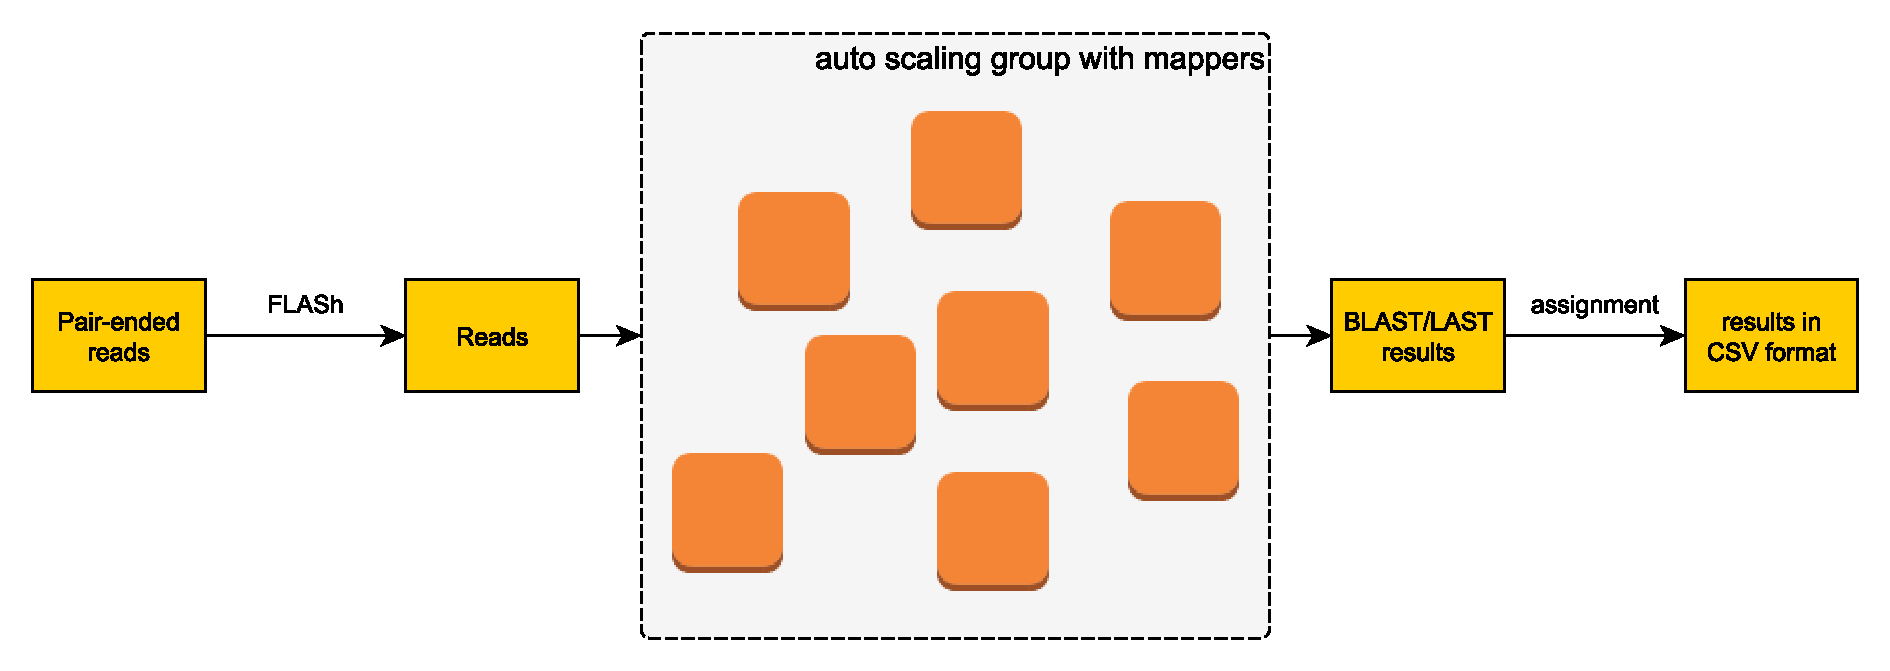
\includegraphics[width=\textwidth]{pipeline_dist.pdf}
\end{frame}

%\end{itemize}

%\begin{frame}
%\frametitle{Cloud solution. Data management}
%Besides computations Metapasta uses AWS for all data management:
%\begin{itemize}
%  \item Reads from samples (S3)
%  \item Taxonomy assignment tables and trees in PDF (S3)
%  \item Metapasta can upload all reads (with assignments) to DynamoDB table.
%\end{itemize}
%\end{frame}



\begin{frame}
\frametitle{Compota}
Compota is a Scala library for performing computations in Amazon cloud:
\begin{itemize}
  \item easy to use (only AWS account is needed)
  \item designed to be \textit{fault tolerant} -- failures in particular nodes never affect the result
  \item \textit{scalable} -- unlimited number of computational nodes can be used with minimal communication overhead.
  % \item Designed to provide maximal level of scalability and availability 
  % (in case of Metapasta it means that it can process {\bf with a good performance} as many data as needed, and never will lose any of reads).
\end{itemize}
\end{frame}


\begin{frame}
\frametitle{Compota. Architecture}
\hspace{0.05\textwidth}
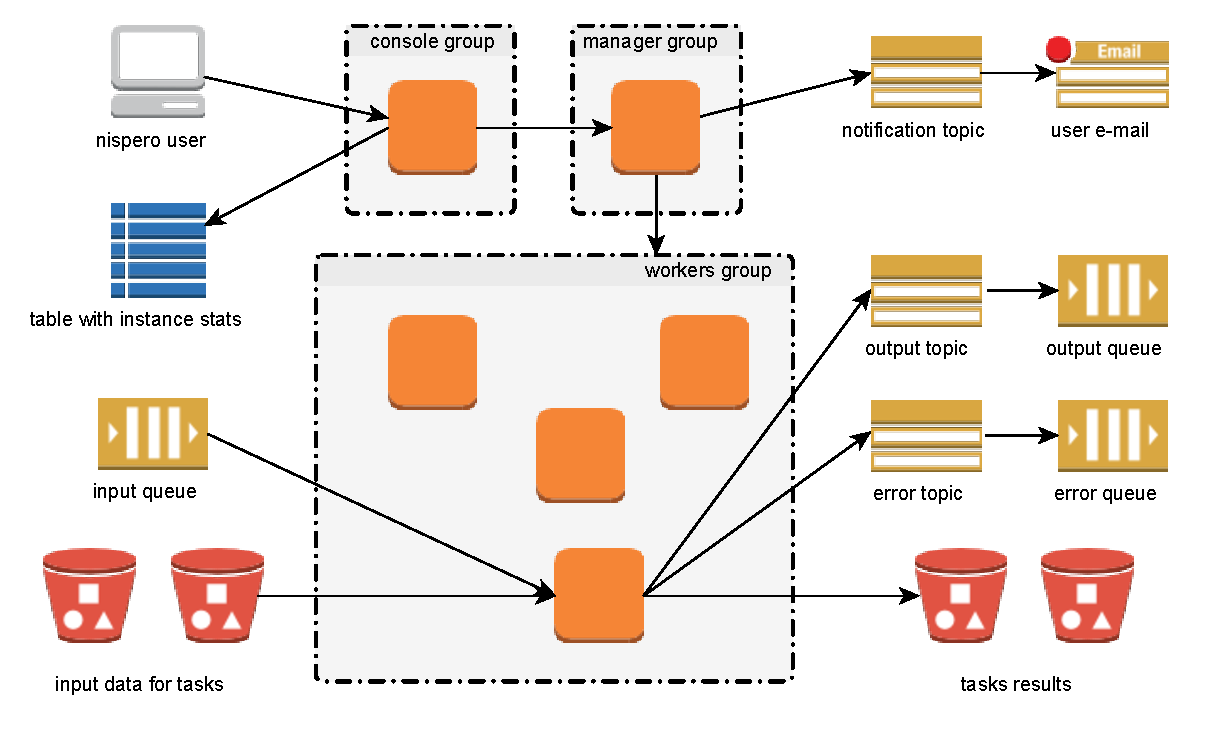
\includegraphics[width=0.9\textwidth]{architecture.pdf}
\hspace{0.05\textwidth}
%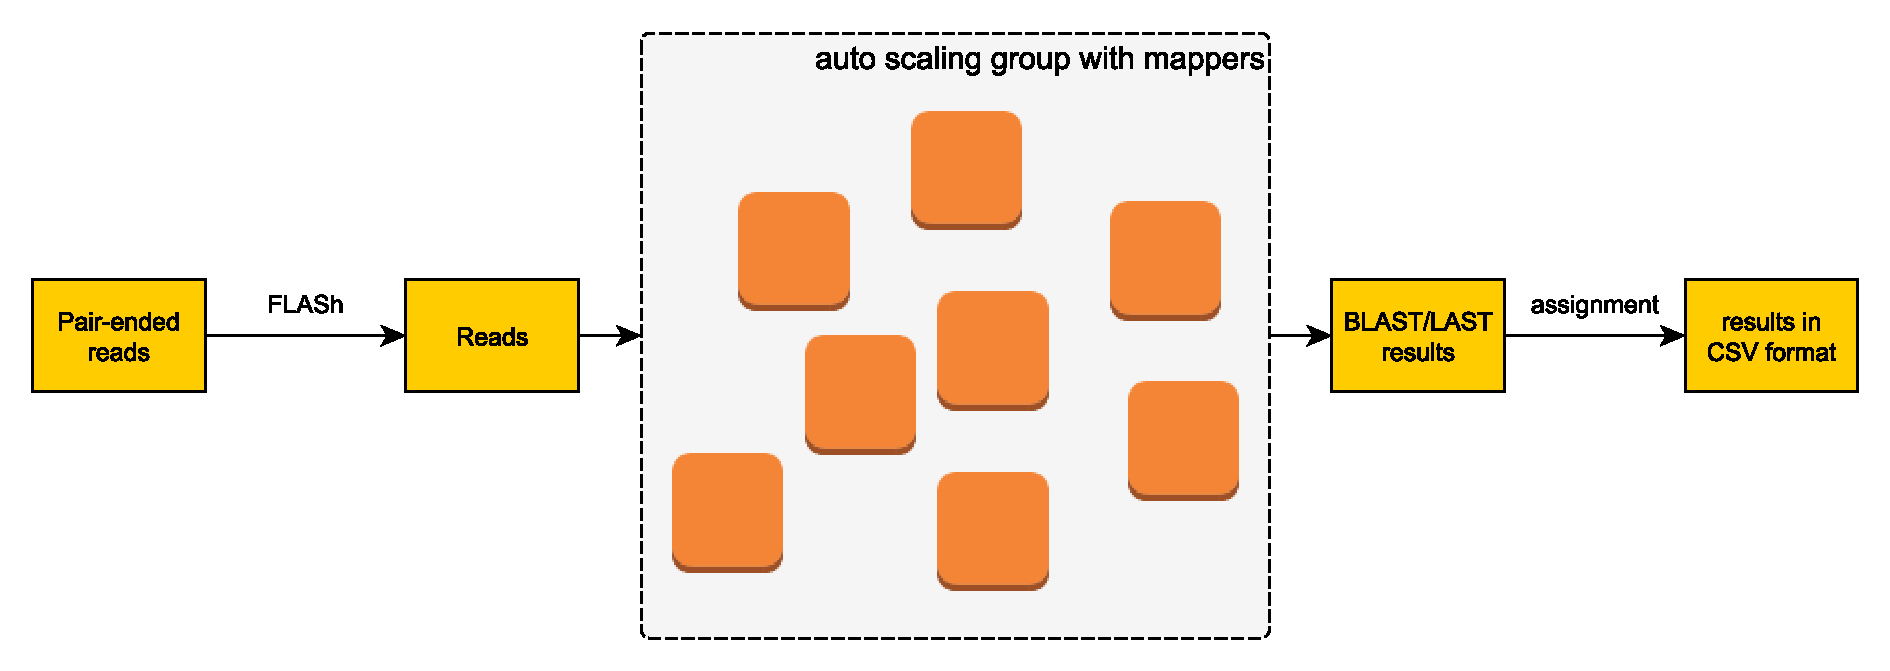
\includegraphics[width=\textwidth]{pipeline_dist.pdf}

\end{frame}

\begin{frame}
\frametitle{Compota. Monoids}

We are using monoid morphisms to describe computations in Compota:

\begin{itemize}
  \item express distributiveness $f(a) = merge(f(split(a)))= merge(f(a_1), f(a_2), \ldots)$
  \item can be composed in pipelines:
\end{itemize}
$$Reads \otimes Reads \xrightarrow{merge} Reads \xrightarrow{BLAST} AssignTable \otimes Reads.$$



\end{frame}



\begin{frame}
\frametitle{Metapasta pipeline}
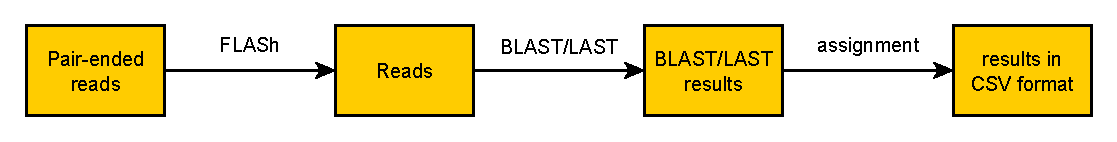
\includegraphics[width=\textwidth]{general.pdf}

\begin{itemize}
  \item (Optional) FLASh merging paired-end reads into bigger reads
  \item mapping reads against the 16S database (with BLAST or LAST)
  \item assignment to the taxonomy tree using Bio4j.
\end{itemize}
\end{frame}

\begin{frame}
\frametitle{Assignment}
Results of \textit{mapping} step:
\begin{itemize}
  \item $read_1 \mapsto \{(taxon^1_1, score^1_1), (taxon^1_2, score^1_2)\}$ 
  \item $read_2 \mapsto \{(taxon^2_1, score^2_1), (taxon^2_2, score^2_2), (taxon^1_3, score^1_3)\}$ 
  \item $read_3 \mapsto \{\}$ 
  \item $read_4 \mapsto \{taxon^4_1\}$ 
\end{itemize}
\vspace{1em}
We assign reads to taxonomy tree using to independent algorithms:
\begin{itemize}
  \item BBH -- Best blast hit
  \item LCA -- Lowest common ancestor.
\end{itemize}
 
\end{frame}

\begin{frame}
\frametitle{Results. Trees}
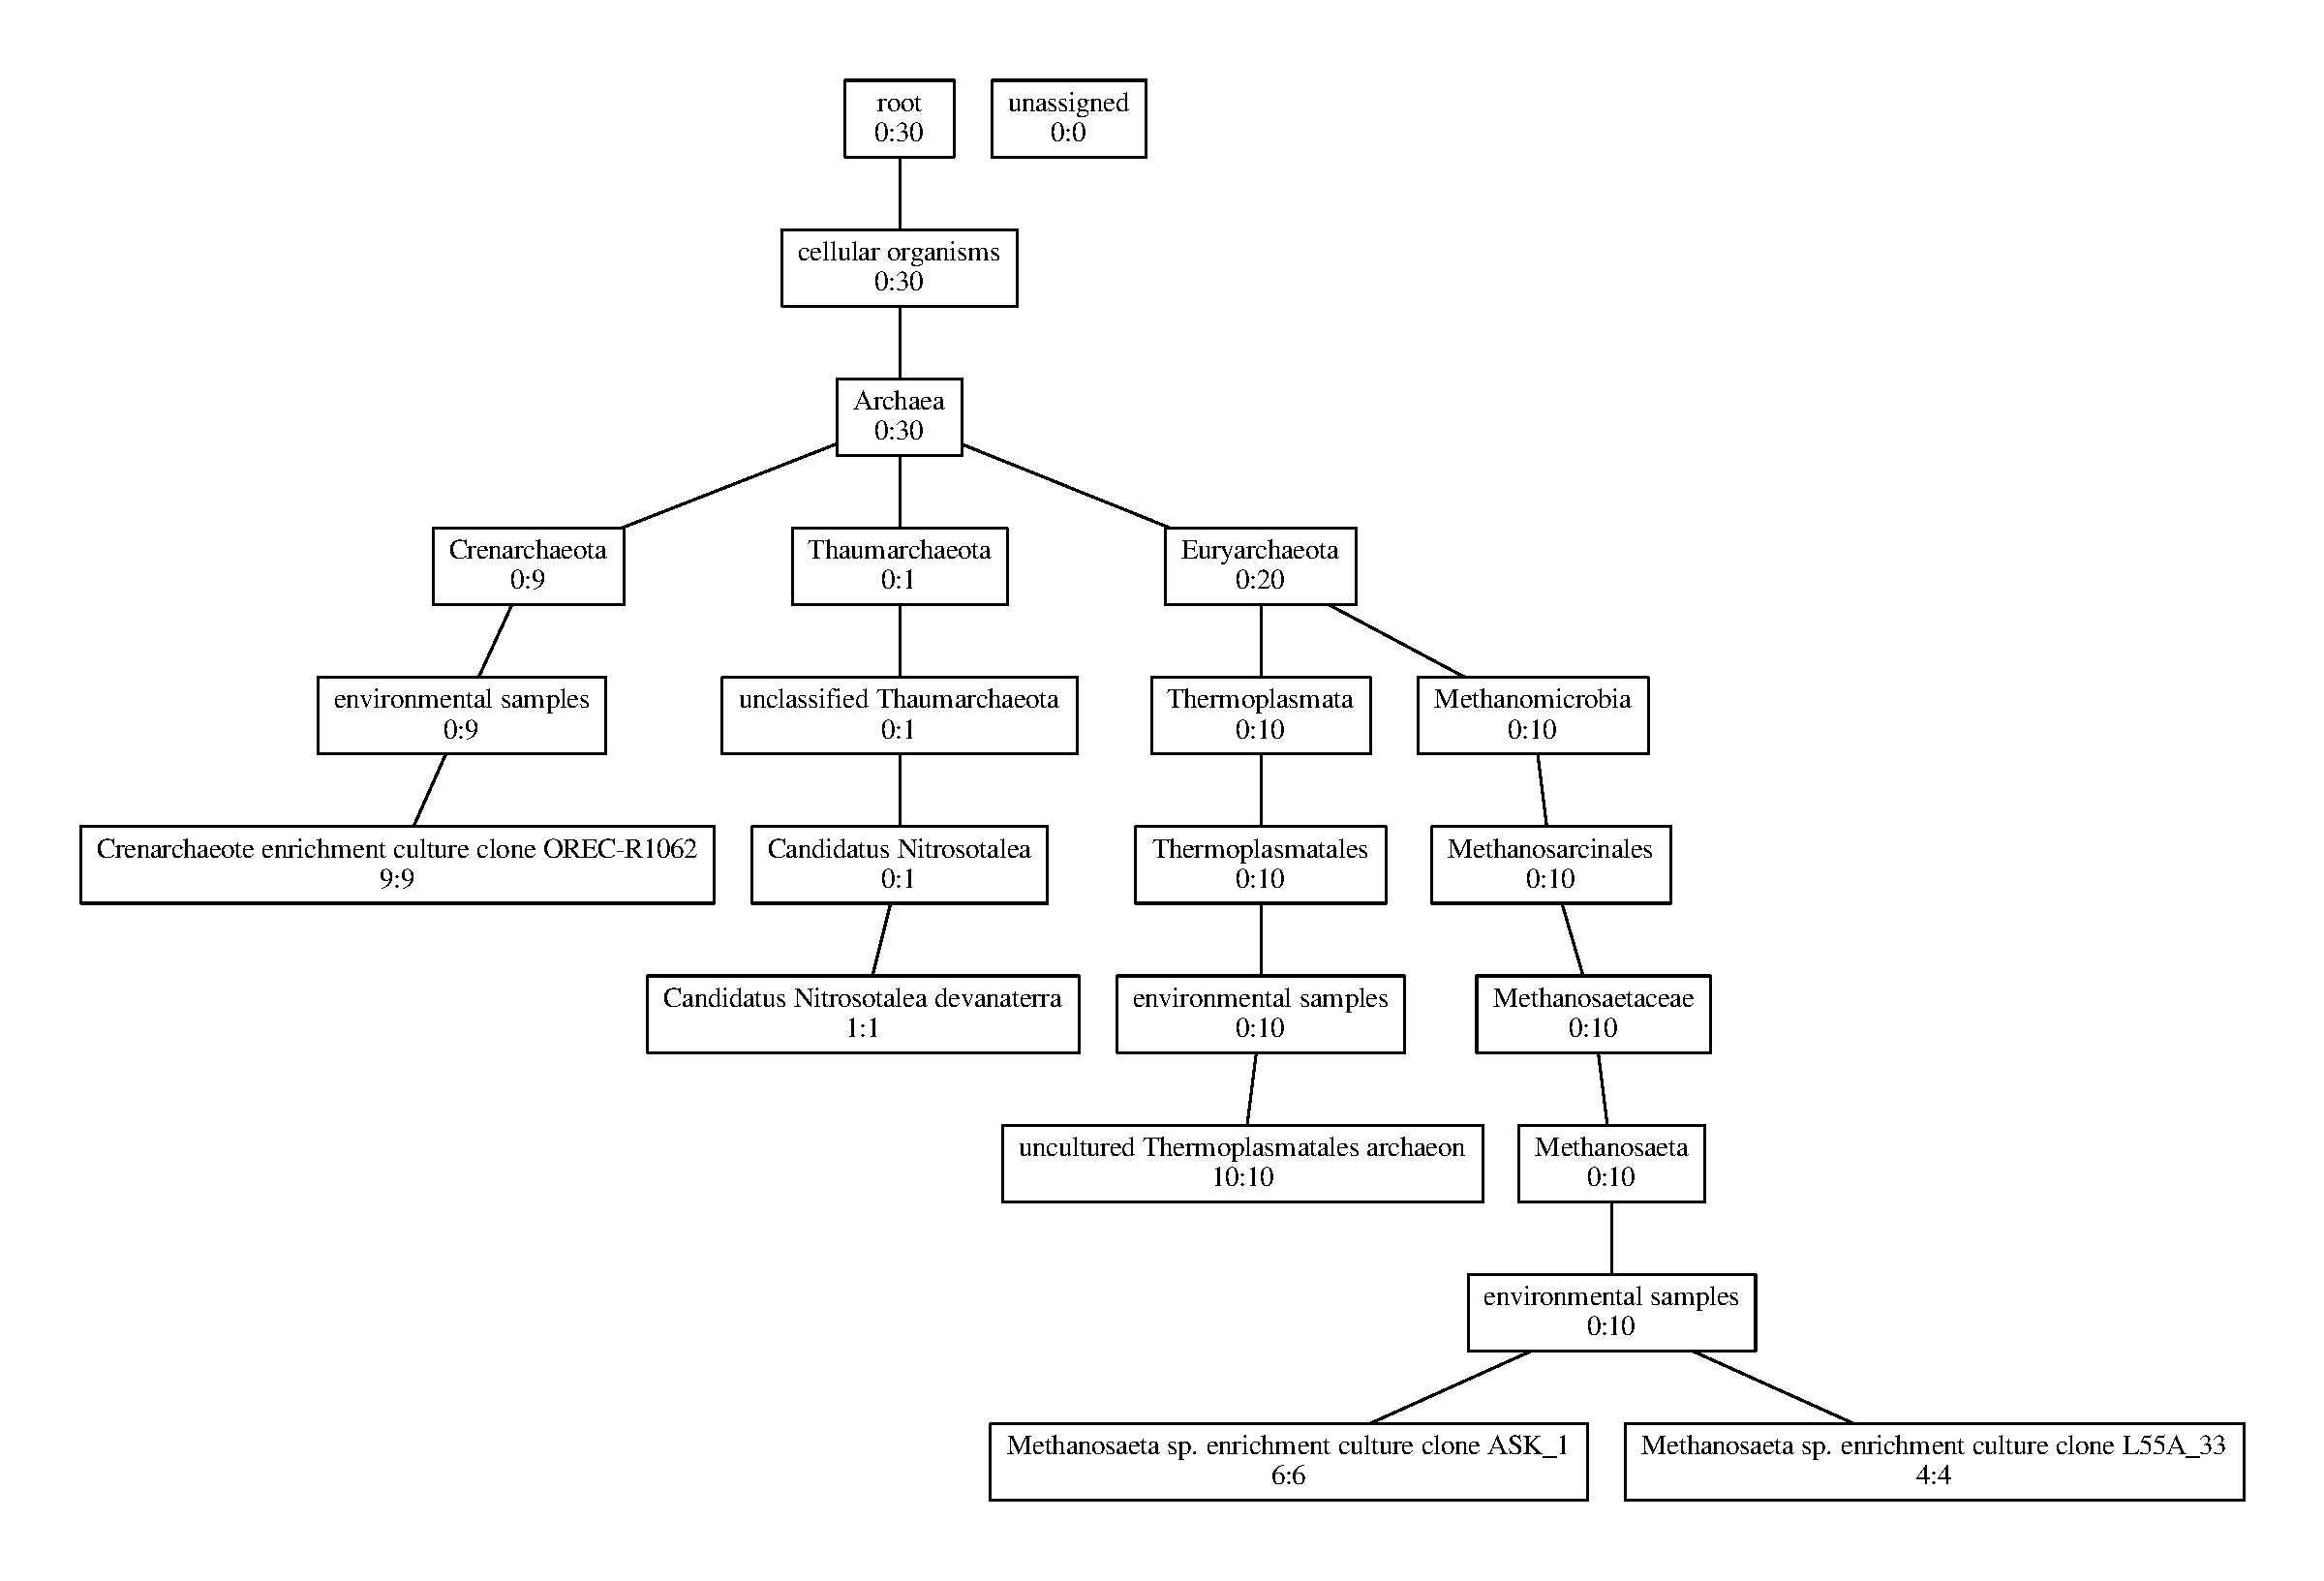
\includegraphics[width=0.9\textwidth]{tree.pdf}
\end{frame}


\begin{frame}
\frametitle{Results. CSV tables}
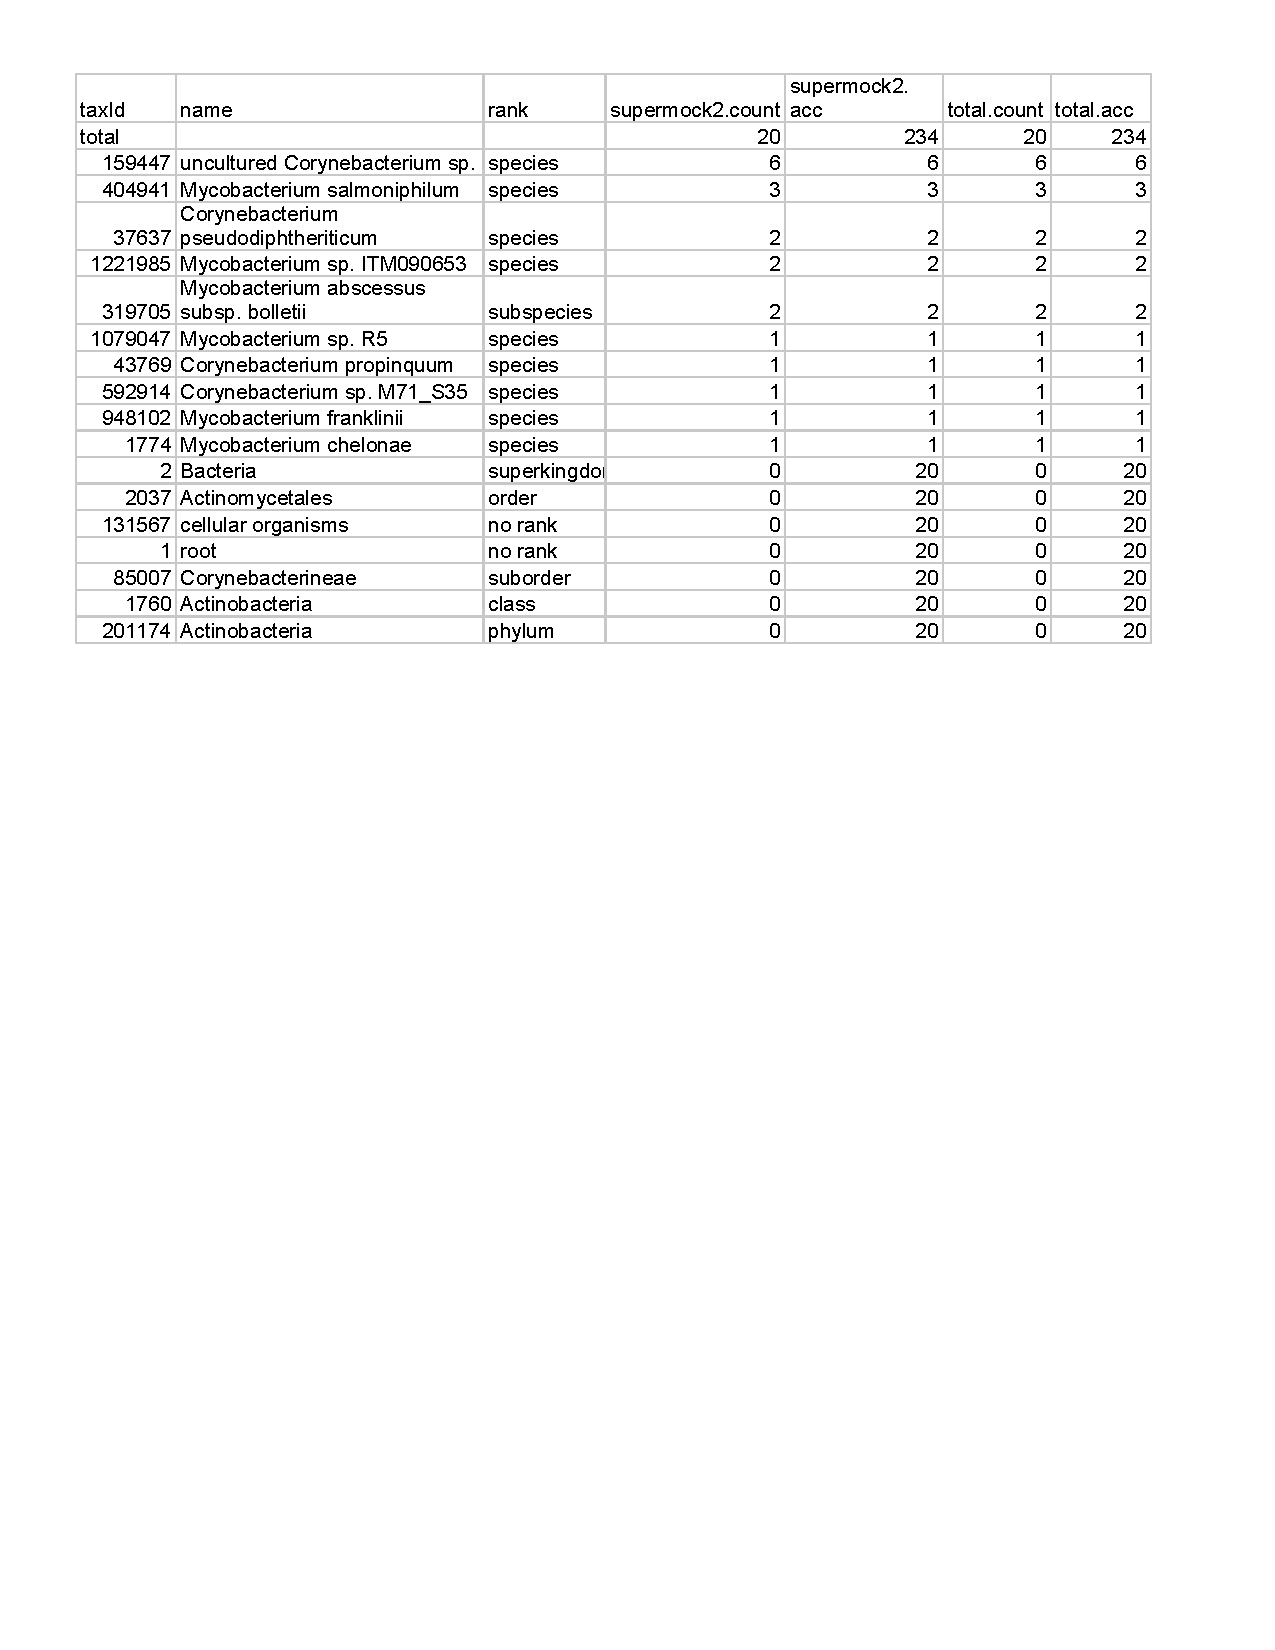
\includegraphics[width=\textwidth]{table.pdf}
\end{frame}



% \begin{frame}
% \frametitle{Nispero}

% \begin{itemize}
%   \item Amazon auto scaling groups
%   \item SQS queues
% \end{itemize}
% \end{frame}

%\begin{frame}
%\frametitle{Input of Metapasta}
%\begin{itemize}
%  \item Sequenced metagenomics samples -- reads in FASTQ format
%  \item Taxonomy database (we are using NCBI taxonomy database that is integrated to Bio4j)
%  \item 16S database (by default Metapasta uses NCBI 16S with some filtering).
%\end{itemize}
%\end{frame}


%\begin{frame}
%\frametitle{Output}
%As result Metapasta produces:
%\begin{itemize}
%  \item for every sample:
%  \begin{itemize}
%  	\item presented taxa with their percentages
%  	\item distribution of assignments on every taxonomy level (kind, genus etc)
%  \end{itemize} 
%  \item aggregated data by samples, group of samples. 
%\end{itemize}
%\end{frame}








%lastvizmeta010-snapshot
% \begin{frame}
% \frametitle{Bio4j}

% \begin{columns}[T]
% 		\begin{column}{.5\textwidth}
% 			
\includegraphics[width=\textwidth]{bio4j.png}
% 		\end{column}
% 		\begin{column}{.5\textwidth}
% 			NCBI taxonomy
% 		\end{column}
% 	\end{columns}
% \end{frame}



 \begin{frame}
 \frametitle{Availability}

\hspace{.35\textwidth}
\includegraphics[width=0.3\textwidth]{agpl.pdf}\hspace{.35\textwidth} \\
 \vspace{1em}
Compota is an open-source project released under AGPLv3 license.
The source code is available at \url{github.com/ohnosequences/metapasta}.

\end{frame}

 \begin{frame}
 \frametitle{INTERCROSSING}
 This project is funded in part by the ITN FP7 project INTERCROSSING (Grant 289974).
 \begin{columns}[T]
 		\begin{column}{.5\textwidth}
 			\hspace{.25\textwidth}
\includegraphics[width=.5\textwidth]{intercrossing.png}
 		\end{column}
 		\begin{column}{.5\textwidth}
 			\hspace{.25\textwidth}\includegraphics[width=.5\textwidth]{mc.jpg}
 		\end{column}
 	\end{columns}
 \end{frame}


\begin{frame}
\Huge{\centerline{Thank you for your attention!}}
\end{frame}
\end{document}